\chapter{Szablony raportów w systemie LaTeX}
\label{ch:szablonyraportowwsystemielatex}

W tym rozdziale przedstawiony zostanie proces przygotowania szablonów dokumentów potrzebnych przy rekrutacji na uczelni PWSZ Nowy Sącz. Opisane zostaną tylko problemy wynikające z tworzenia automatycznie uzupełnianych szablonów oraz ich rozwiązania. Wszystkie stworzone szablony znajdują się w załączniku 3 w katalogu \texttt{template/}.

\section{Idea tworzenia szablonów}

Do wszystkich tych dokumentów potrzebny jest szablon w języku oprogramowania do zautomatyzowanego składu tekstu. W tej pracy został wybrany program LaTeX ze względu na jego możliwości automatyzacji procesu parsowania danych i uzupełniania nimi danych miejsc w tekście.
\par Stworzenie szablonów polega, więc na wcześniejszym przygotowaniu plików tex, zawierających wcześniej strukturę danego dokumentu z ''pustymi''  miejscami do uzupełnienia przez program. Do uzupełnienia tych miejsc można wykorzystać funkcję LaTeX'u jaką jest tworzenie nowych poleceń z parametrami, gdzie odpowiednio parametry te będą wartościami, które zostaną wpisane w dane miejsce w danym dokumencie. Następnie wystarczy wywołać daną komendę z odpowiednimi wartościami aby otrzymać uzupełniony dokument. Dane polecenie możemy wywoływać wielokrotnie od różnych wartości tworząc w ten sposób wiele dokumentów tego samego typu o różnych zmiennych wartościach takich jak np imię i nazwisko. 
\par Do wytworzenia wywołań tych komend posłuży oddzielny program. Poprzez dodanie zapytania SQL w odpowiedniej formule do plików tex. Program \emph{DBLatexRaport} wyszuka takie zapytanie i uzupełni szablon wywołaniami poleceń z wartościami parametrów, jakimi będą wartości pola z rekordów zapytania SQL. 

\section{Środowisko kompilacji raportów}

Środowisko do kompilacji dokumentów zostało specjalnie przygotowane poprzez usuniecie nadmiarowych (nieużywanych) bibliotek. Dzięki temu cały system będzie zajmował mniej pamięci na dysku twardym i będzie łatwiejsze do przenoszenia. Dodatkowo kompilatora nie trzeba instalować, dzięki czemu cały system będzie szybki w użyciu. Środowisko kompilacji wymaga systemu operacyjnego Windows. Środowisko to znajduje się w załączniku 3. razem z programem.


\section{Tworzenie szablonów raportów do systemu rekrutacji}

W rekrutacji na uczelnie wykorzystuje się dokumenty, które należało dokładnie odwzorować w nowym systemie. Są to następujące dokumenty:\\
\begin{enumerate}
\item protokół przekazania
\item listy potwierdzenia podjęcia studiów 
\item listy rankingowe 
\item listy przyjętych
\item listy nieprzyjętych
\item decyzja o przyjęciu danego kandydata
\item decyzja o nieprzyjęciu danego kandydata 
\end{enumerate}
\vspace{5mm}
\par
Przy tworzeniu szablonów wystąpiły problemy, które należało rozwiązać.  W dużej mierze problemy te powtarzają się,  opisane więc zostały tylko rozwiązania tych problemów a nie każdy szablon raportu. W poniższych podsekcjach znajdują się przedstawione problemy oraz ich rozwiązania. W celu dokładnego sprawdzenia wykonania danego szablonu, wszystkie powyższe szablony zostały dołączone w załączniku 3 do wglądu.
\subsection{Definiowanie zmiennych}

Pewne dynamicznie pobrane z bazy danych informacje powtarzają się w szablonach w wielu miejscach, zaistniała więc potrzeba zapisania tych informacji jednorazowo do zmiennych, które można wywołać w każdym miejscu w dokumencie. 
\par
Do uzyskania takiego efektu wykorzystana została poniższa procedura:
 \begin{lstlisting}
\long\def\parametrRekrutacyjny#1#2{\expandafter\def\csname#1\endcsname{#2}}
 \end{lstlisting}
Każde wywołanie polecenia \texttt{parametrRekrutacyjny} utworzy zmienną, której nazwą będzie parametr pierwszy, natomiast wartością zwracaną drugi.
\par 
Po wywołaniu przykładowych danych pokazanych poniżej:
 \begin{lstlisting}
\parametrRekrutacyjny{dataWydaniaDecyzji}{2015-03-06}
\parametrRekrutacyjny{miejsceWydaniaDecyzji}{Nowy Sącz}
\parametrRekrutacyjny{przewodniczacyIKR}{dr inż. Tomasz Kądziołka}
 \end{lstlisting}
będzie można pobrać te zmienne za pomocą wywołania komendy o nazwie 1 parametru. Wywołanie więc \texttt{ \textbackslash dataWydaniaDecyzji} zwróci wartość w danym miejscu \texttt{2015-03-06}.

\subsection{Wstawianie wartości}

Zapewnienie wygodnego użytkowania szablonu wymaga wcześniejszej deklaracji zmiennych zaraz po deklaracji komendy. Wszystkie parametry przekazane przy wywołaniu polecenia, przekazywane są pod postacią \texttt{\#numer}, więc aby zapewnić przejrzyste i proste wykorzystanie tych parametrów, można zdefiniować z nich zmienne wewnątrz tej komendy i odwoływać się do nich poprzez nazwy, a nie cyfry:

 \begin{lstlisting}
\providecommand{\decyzjaSingle}{}\renewcommand{\decyzjaSingle}[9]{
\providecommand{\liczbaPunktow}{}\renewcommand{\liczbaPunktow}{#1}
\providecommand{\decyzjaNumer}{}\renewcommand{\decyzjaNumer}{#2}
\providecommand{\nazwiskoImie}{}\renewcommand{\nazwiskoImie}{#3}
\providecommand{\adresI}{}\renewcommand{\adresI}{#4}
\providecommand{\adresII}{}\renewcommand{\adresII}{#5}
\providecommand{\nrTeczkiKodKierunku}{}\renewcommand{\nrTeczkiKodKierunku}{#6}
\providecommand{\czyPrzyjety}{}\renewcommand{\czyPrzyjety}{#7}
\providecommand{\dataPrzyjeciaPodania}{}\renewcommand{\dataPrzyjeciaPodania}{#8}
\providecommand{\MenKobieta}{}\renewcommand{\MenKobieta}{#9}
\def\panpani#1#2{\if\MenKobieta M#1\else #2\fi}
 \end{lstlisting}
 
Przykładowy kawałek kodu źródłowego szablonu w którym wykorzystane zostały zmienne przekazane przez parametry komendy:
 \begin{lstlisting}
...
\begin{picture}(190,70)
\put(0,72){\instytutStamp}
\put(120,28){\parbox[t]{9cm}{\textbf{\panpani{Pan}{Pani}}\\[0.2cm]\nazwiskoImie
\\\adresI\\\adresII\\[.2cm]{\footnotesize \nrTeczkiKodKierunku}}}
%\put(-10,0){\line(1,0){5}}\put(195,0){\line(1,0){5}}
\end{picture}
}
...
 \end{lstlisting}

Dla  każdego wywołania komendy o nazwie \texttt{decyzjaSingle} od podanych parametrów, wyświetlona zostanie cała zawartość tego tego polecenia oraz podanych wartości w ustalonych miejscach. Dla poniższych wygenerowanych losowo danych, wynik kompilacji pokazany został na rysunku \ref{fig:wstawianie}. Pełny kod szablonu znajduje się w załączniku 3 w pliku \texttt{template/decycja.tex}.
 \begin{lstlisting}
\decyzja{38}{328/2015}{ Ablewicz Monika}{ gen.Stefana Grota-Roweckiego 8}
{Nowy Sacz 33-300}{39 INF-n 1}{2}{14.08.2015}{K}
 \end{lstlisting}
 
 
 
\begin{figure}
    \centering
    
\includegraphics[width=0.8\textwidth]{rys/szablony/wstawianie.png}
    \caption{Przykład rozwiązania wstawiania wartości w szablonie}
    \label{fig:wstawianie}
\end{figure}



 
 \subsection{Wyświetlanie listy}
Problem występujący w protokole przekazania oraz we wszystkich listach. Dla przykładu potrzeba wyświetlić poniższą listę w tabeli, gdzie wartości pochodzą z bazy danych:
\begin{lstlisting}
Lp. Tok studiów Liczba kopert
1 Informatyka — niestacjonarne STUDIA pierwszego stopnia 1455
2 Informatyka — stacjonarne STUDIA pierwszego stopnia 729
3 Mechatronika — niestacjonarne STUDIA pierwszego stopnia 1447
...
\end{lstlisting}
\vspace{5mm}
\par
Stworzenie tabeli wymaga dodatkowo stworzenia nagłówka tabeli i zakończenia tabeli. Cała zawartość listy, czyli wywołania komend  od parametrów zawierających rekordy z bazy danych, powinna znaleźć się pomiędzy nagłówkiem a zakończeniem. W tym celu program \emph{DBLatexRaport} został rozwinięty o dodatkową funkcjonalność, która pozwala na dodawanie selekcji danych wewnątrz szablonu, co ułatwia stworzenie listy. 
\par
Do wyświetlenia jednego wiersza posłuży komenda \texttt{prodokolprzekazania}:
\vspace{5mm}
\begin{lstlisting}
\newcommand{\protokolprzekazania}[2]{\stepcounter{lp}\thelp&{\tiny #1}&#2\\}
\end{lstlisting}
\vspace{3mm}
\par
Następnie wywoływanie tego polecenia od podanych parametrów pomiędzy rozpoczęciem i zakończeniem tabeli spowoduje, że utworzona zostanie tabela zawierająca wszystkie rekordy pobrane z bazy. Wynik kodu można zobaczyć na rysunku \ref{fig:lista}.
\begin{lstlisting}
\begin{center}
\begin{tabular}{clc}
\hline
Lp.&\multicolumn{1}{c}{Tok studiów}&Liczba kopert\\
\hline

\protokolprzekazania{Informatyka --- niestacjonarne STUDIA pierwszego stopnia}{1455}
\protokolprzekazania{Informatyka --- stacjonarne STUDIA pierwszego stopnia}{729}
\protokolprzekazania{Mechatronika --- niestacjonarne STUDIA pierwszego stopnia}{1447}
...

\hline\end{tabular}\end{center}
\end{lstlisting}

\begin{figure}[h]
    \centering
      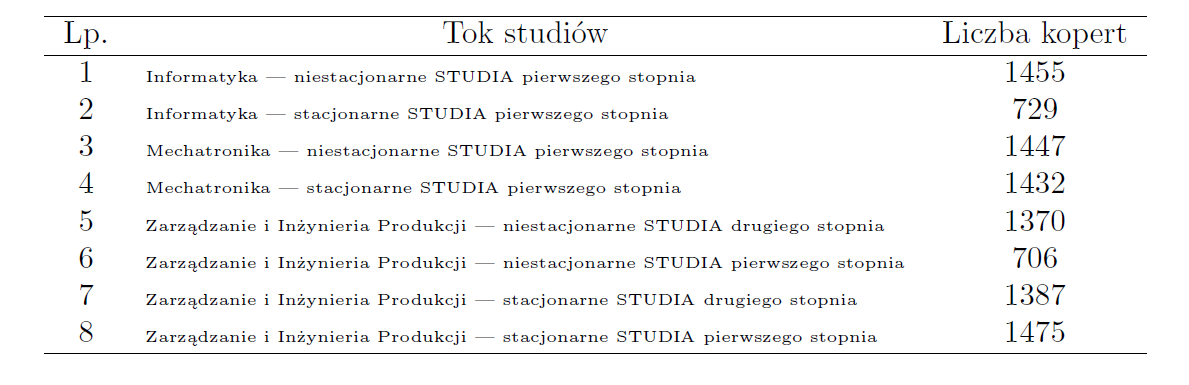
\includegraphics[width=0.8\textwidth]{rys/szablony/lista.png}
    \caption{Przykład rozwiązania problemu wyświetlania listy}
     \label{fig:lista}
\end{figure}

\subsection{Grupowanie}

Problem grupowania występował przy tworzeniu list kandydatów dla różnych toków nauki. Dla każdego toku automatycznie musiała powstać oddzielna lista. Dla każdej listy także nagłówki posiadały różne wartości. 
\par Rozwiązaniem tego problemu okazało się wykorzystanie przygotowanej na początku komendy \texttt{provideenvironment} tworzącej środowisko, dzięki któremu można utworzyć rozpoczęcie i zakończenie danej grupy. 
\begin{lstlisting}
\makeatletter
\def\provideenvironment{\@star@or@long\provide@environment}
\def\provide@environment#1{%
        \@ifundefined{#1}%
                {\def\reserved@a{\newenvironment{#1}}}%
                {\def\reserved@a{\renewenvironment{dummy@environ}}}%
        \reserved@a
}
\def\dummy@environ{}
\makeatother
\end{lstlisting}
Daje to możliwość tworzenia nagłówków oraz zakończeń dla każdej listy poprzez wywoływanie środowisk od odpowiednich parametrów. Każde środowisko należy zakończyć poprzez wywołanie komendy o nazwie środowiska z prefiksem end.
\vspace{5mm}
\par
Poniżej przedstawiony został przykład wykorzystania pojedynczego grupowania po trzech polach, która został wykorzystany w szablonach przy rekrutacji:

\begin{lstlisting}
\providecommand{\listaprzyjetych}{}\renewcommand{\listaprzyjetych}[1]{\stepcounter{lp}\thelp&#1\\}

\provideenvironment{listaprzyjetychA}{}{}
\renewenvironment{listaprzyjetychA}[3]{
\setcounter{lp}{0} 
{\small \begin{tabular}[t]{ll}
Studia:&#1\\
Kierunek studiów:&#2\\
Forma studiów:&#3\\
Rok studiów:&PIERWSZY\\
Rok akademicki:&\rokAkademicki
\end{tabular}}
\begin{center}
\begin{longtable}{|c|l|}
%\hline
%\textbf{Lp.}&\multicolumn{1}{c|}{\textbf{Nazwisko i imiona}}\\\hline 
%\hline
}

{
\hline\end{longtable}\end{center}
}
\end{lstlisting}

Dzięki takiej konstrukcji możliwe będzie automatyczne tworzenie różnych list z dynamicznym nagłówkiem, który przyjmuje wartości w zależności od wywołanych parametrów. Przykład wykorzystania powyższego zapisu znajduje się poniżej (Dane są losowo wygenerowane):

\begin{lstlisting}
\listaprzyjetychA{pierwszego stopnia}{Informatyka}{niestacjonarne}
\listaprzyjetych{ Ablewicz Monika}
\listaprzyjetych{ Abram Halina}
\listaprzyjetych{ Adamczyk Józef}
\endlistaprzyjetychA
\listaprzyjetychA{pierwszego stopnia}{Informatyka}{stacjonarne}
\listaprzyjetych{ Adamczyk Katarzyna}
\listaprzyjetych{ Adamczyk Mieczysław}
\listaprzyjetych{ Adamczyk Stanisław}
\endlistaprzyjetychA
\end{lstlisting}

Tak przygotowane dane powinny utworzyć dokładnie taką ilość list, ile jest wywołań grup. Każda lista powinna posiadać nagłówki z wartościami przekazanymi w parametrach grupy. W tym przypadku będą to dwie listy dla studiów stacjonarnych oraz niestacjonarnych. Zobaczyć to można na rysunku \ref{fig:grupowanie}.
\begin{figure}[h]
    \centering
      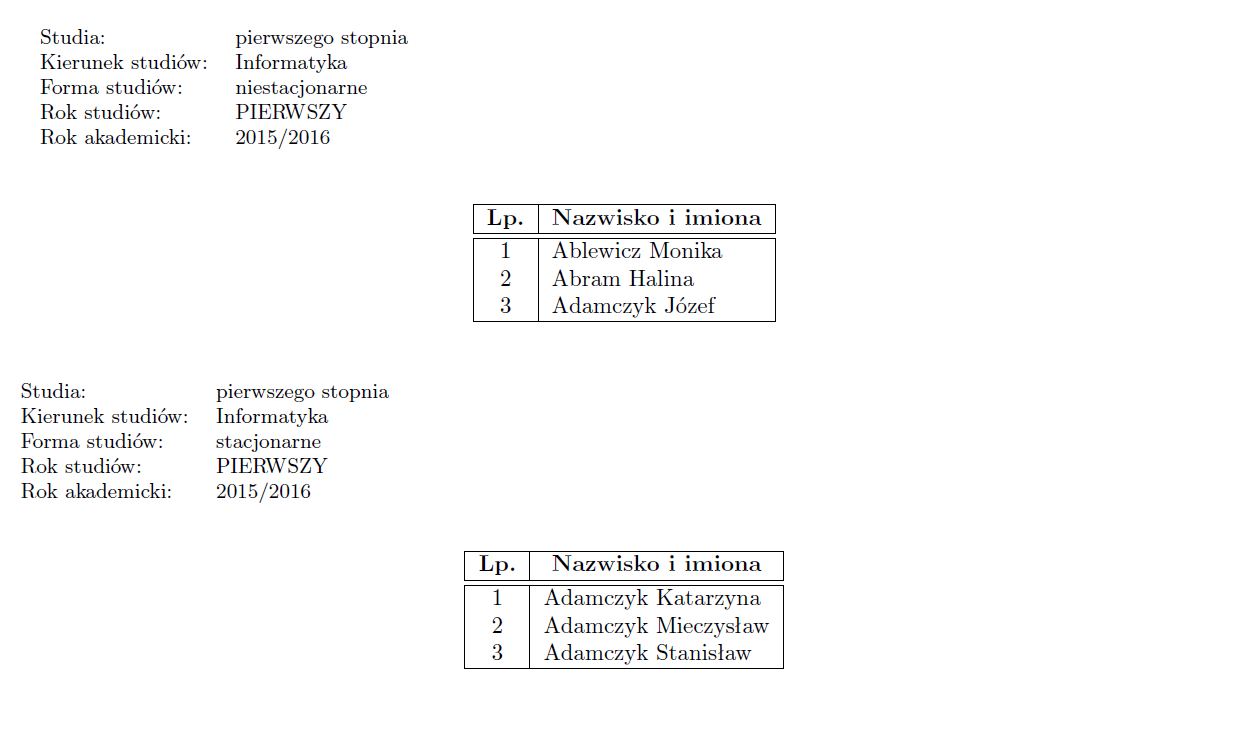
\includegraphics[width=0.8\textwidth]{rys/szablony/grupowanie.png}
    \caption{Przykład rozwiązania problemu grupowania}
     \label{fig:grupowanie}
\end{figure}
\subsection{Nadmierna liczba parametrów}

Środowisko LaTeX posiada ograniczenie, którym jest liczba parametrów komendy, wynosząca dziewięć. Istnienie tego ograniczenia powoduję, iż stworzenie komendy przyjmującej więcej jak 9 wartości staje się problemem. Nietypowym rozwiązaniem tego problemu może być użycie grupowania, które przejmie nadmiar parametrów do wywołań grup w których znajdą się już wywołania komend zwierających nie przepełnioną ilość parametrów. 
\vspace{5mm}
\par
Problem ten wystąpił w szablonie dla decyzji przyjęcia kandydata. Ilość pojedynczych informacji o kandydacie wynosi 12, które należy wstawić w różne miejsca. Liczba ta przekracza limit parametrów komendy w LaTeX'ie. Do rozwiązania problemu wykorzystana została grupa pomocnicza przejmująca 3 pierwsze parametry jakimi są wartości: studia, kierunek oraz forma studiów. Stworzona grupa pomocnicza przy każdym jej wywołaniu ustawiała te wartości pod zmienne, które były identyczne dla wszystkich kandydatów w grupie i następnie zmienne te zostały już użyte w celu wstawiania wartości dla każdego kandydata zawartego w tej grupie. Poniżej znajduje się zapis tworzenia pomocniczej grupy.
\begin{lstlisting}
\provideenvironment{decyzjaA}{}{}
\renewenvironment{decyzjaA}[3]
{
\providecommand{\studia}{}\renewcommand{\studia}{#1}
\providecommand{\kierunekStudiow}{}\renewcommand{\kierunekStudiow}{#2}
\providecommand{\formaStudiow}{}\renewcommand{\formaStudiow}{#3}
}
{} 
\end{lstlisting}

Przykład wykorzystania powyższego zapisu znajduje się poniżej (Dane są losowo wygenerowane) :
\begin{lstlisting}
\decyzjaA{pierwszego stopnia}{Informatyka}{niestacjonarne}
\decyzja{38}{328/2015}{ Ablewicz Monika}{ gen.Stefana Grota-Roweckiego 8}
{Nowy Sacz 33-300}{39 INF-n 1}{2}{14.08.2015}{K}
...
\enddecyzjaA
\end{lstlisting}
